\chapter{Final Results and Conclusions}
\label{sec:results}
\section{Analysis of each plane}
\begin{figure}
    \centering
    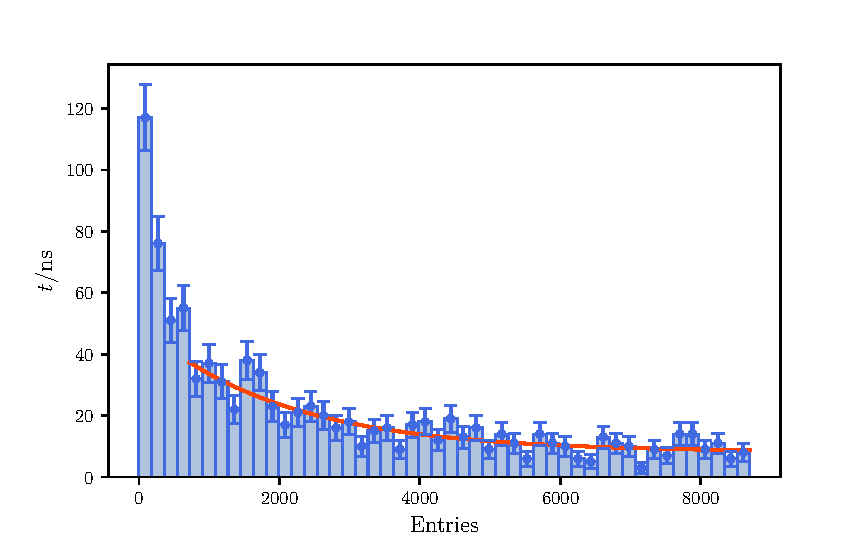
\includegraphics[width=0.6\textwidth]{plots/p0.pdf}
    \caption{Plane 0.}
    \label{fig:p0}
\end{figure}
\begin{figure}
    \centering
    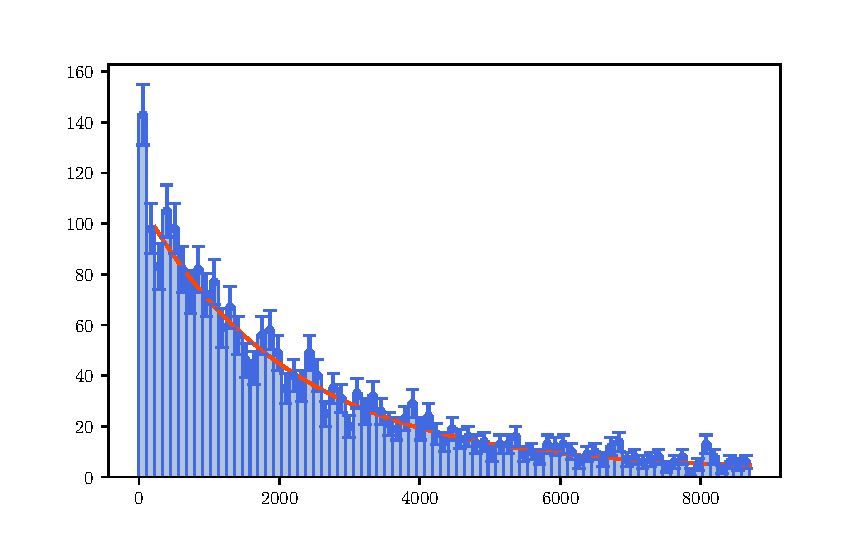
\includegraphics[width=0.6\textwidth]{plots/p1.pdf}
    \caption{Plane 1.}
    \label{fig:p1}
\end{figure}
\begin{figure}
    \centering
    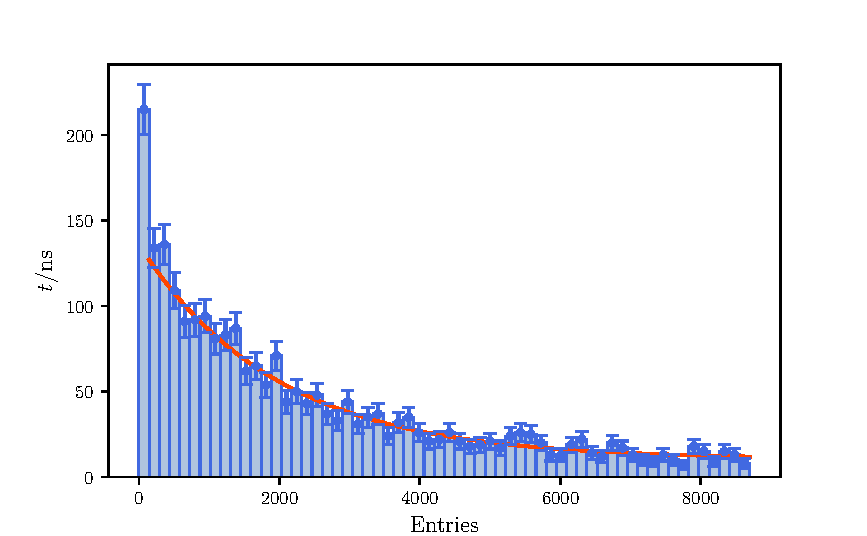
\includegraphics[width=0.6\textwidth]{plots/p2.pdf}
    \caption{Plane 2.}
    \label{fig:p2}
\end{figure}
Fit function:
\begin{equation*}
    N = a \cdot \exp(- \frac{t}{\tau}) + b
\end{equation*}
with N as the number of counts.
Parameters in Table.
\begin{table}[!htp]
    \centering
    \caption{Parameters of the Data analysis fits.}
    \label{tab:data}
    \begin{tabular}{c | c c c c | c}
    \toprule
    {Plane} & {Entries} & {Parameter $a$} &{Parameter $b$} & {Lifetime $\tau / \symup{\mu s}$} & {$\chi^2/\symup{d.o.f.}$} \\
    \midrule
    P0 & 1030 & 41 \pm 5 & 8 \pm 2 & 2.0 \pm 0.4 & 1.085 \\
    P1 & 2345 & 108 \pm 3 & 4 \pm 1 & 2.1 \pm 0.1 & 0.893 \\
    P2 & 2510 & 125 \pm 5 & 10 \pm 2 & 2.0 \pm 0.1 & 0.923  \\
    P1 + P2 + P3 & 5885 & 400 \pm 11 & 30 \pm 4 & 2.1 \pm 0.1 & 0.959 \\
    \bottomrule
    \end{tabular}
    \end{table} 

\section{All planes}
\begin{figure}
    \centering
    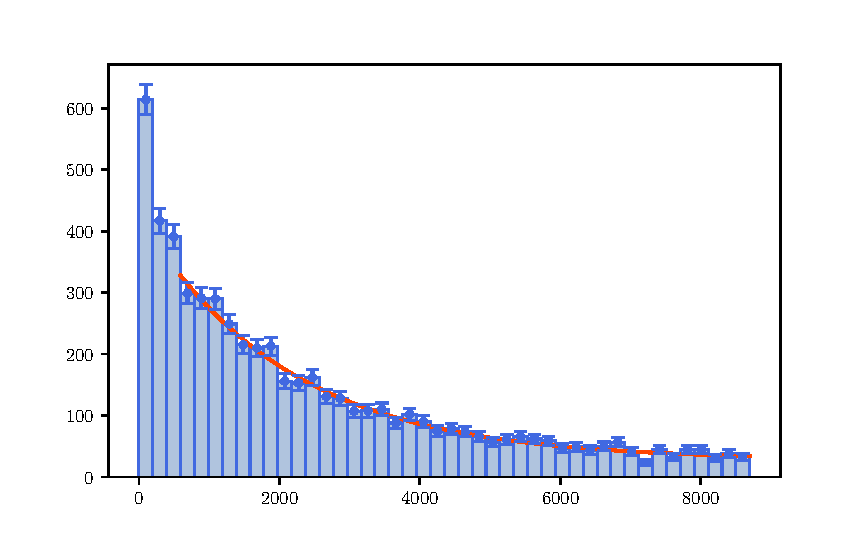
\includegraphics[width=0.6\textwidth]{plots/pALL.pdf}
    \caption{All Planes.}
    \label{fig:pALL}
\end{figure}

\section{With bound Muons}

\begin{figure}
    \centering
    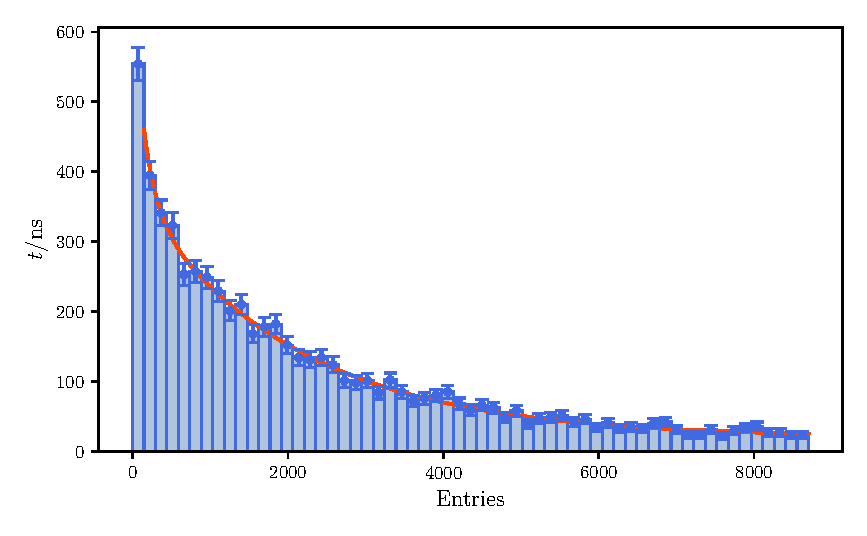
\includegraphics[width=0.6\textwidth]{plots/ptest.pdf}
    \caption{All Planes with bound Muons.}
    \label{fig:ptest}
\end{figure}

Parameters:
\begin{align*}
    a &= 228 \pm 13 \\
    b &= 21 \pm 2 \\
    \tau_{\text{free}} &= 2.1 \pm 0.1 \; \mu s\\
    \tau_{\text{bound}} &= 0.21 \pm 0.06 \;\mu s
\end{align*}